% Requires \usepackage{tikz} in the preamble. The TikZ libraries are
% loaded here so the figure works even if the preamble omits them.
\usetikzlibrary{arrows.meta,positioning,backgrounds,fit}
\begin{figure}[!htbp]
\centering
\definecolor{kgproc}{HTML}{C8691C}
\definecolor{kgmat}{HTML}{2F6F9F}
\definecolor{kgdata}{HTML}{3F8B45}
\definecolor{kgqual}{HTML}{7D4E9E}
\resizebox{\textwidth}{!}{%
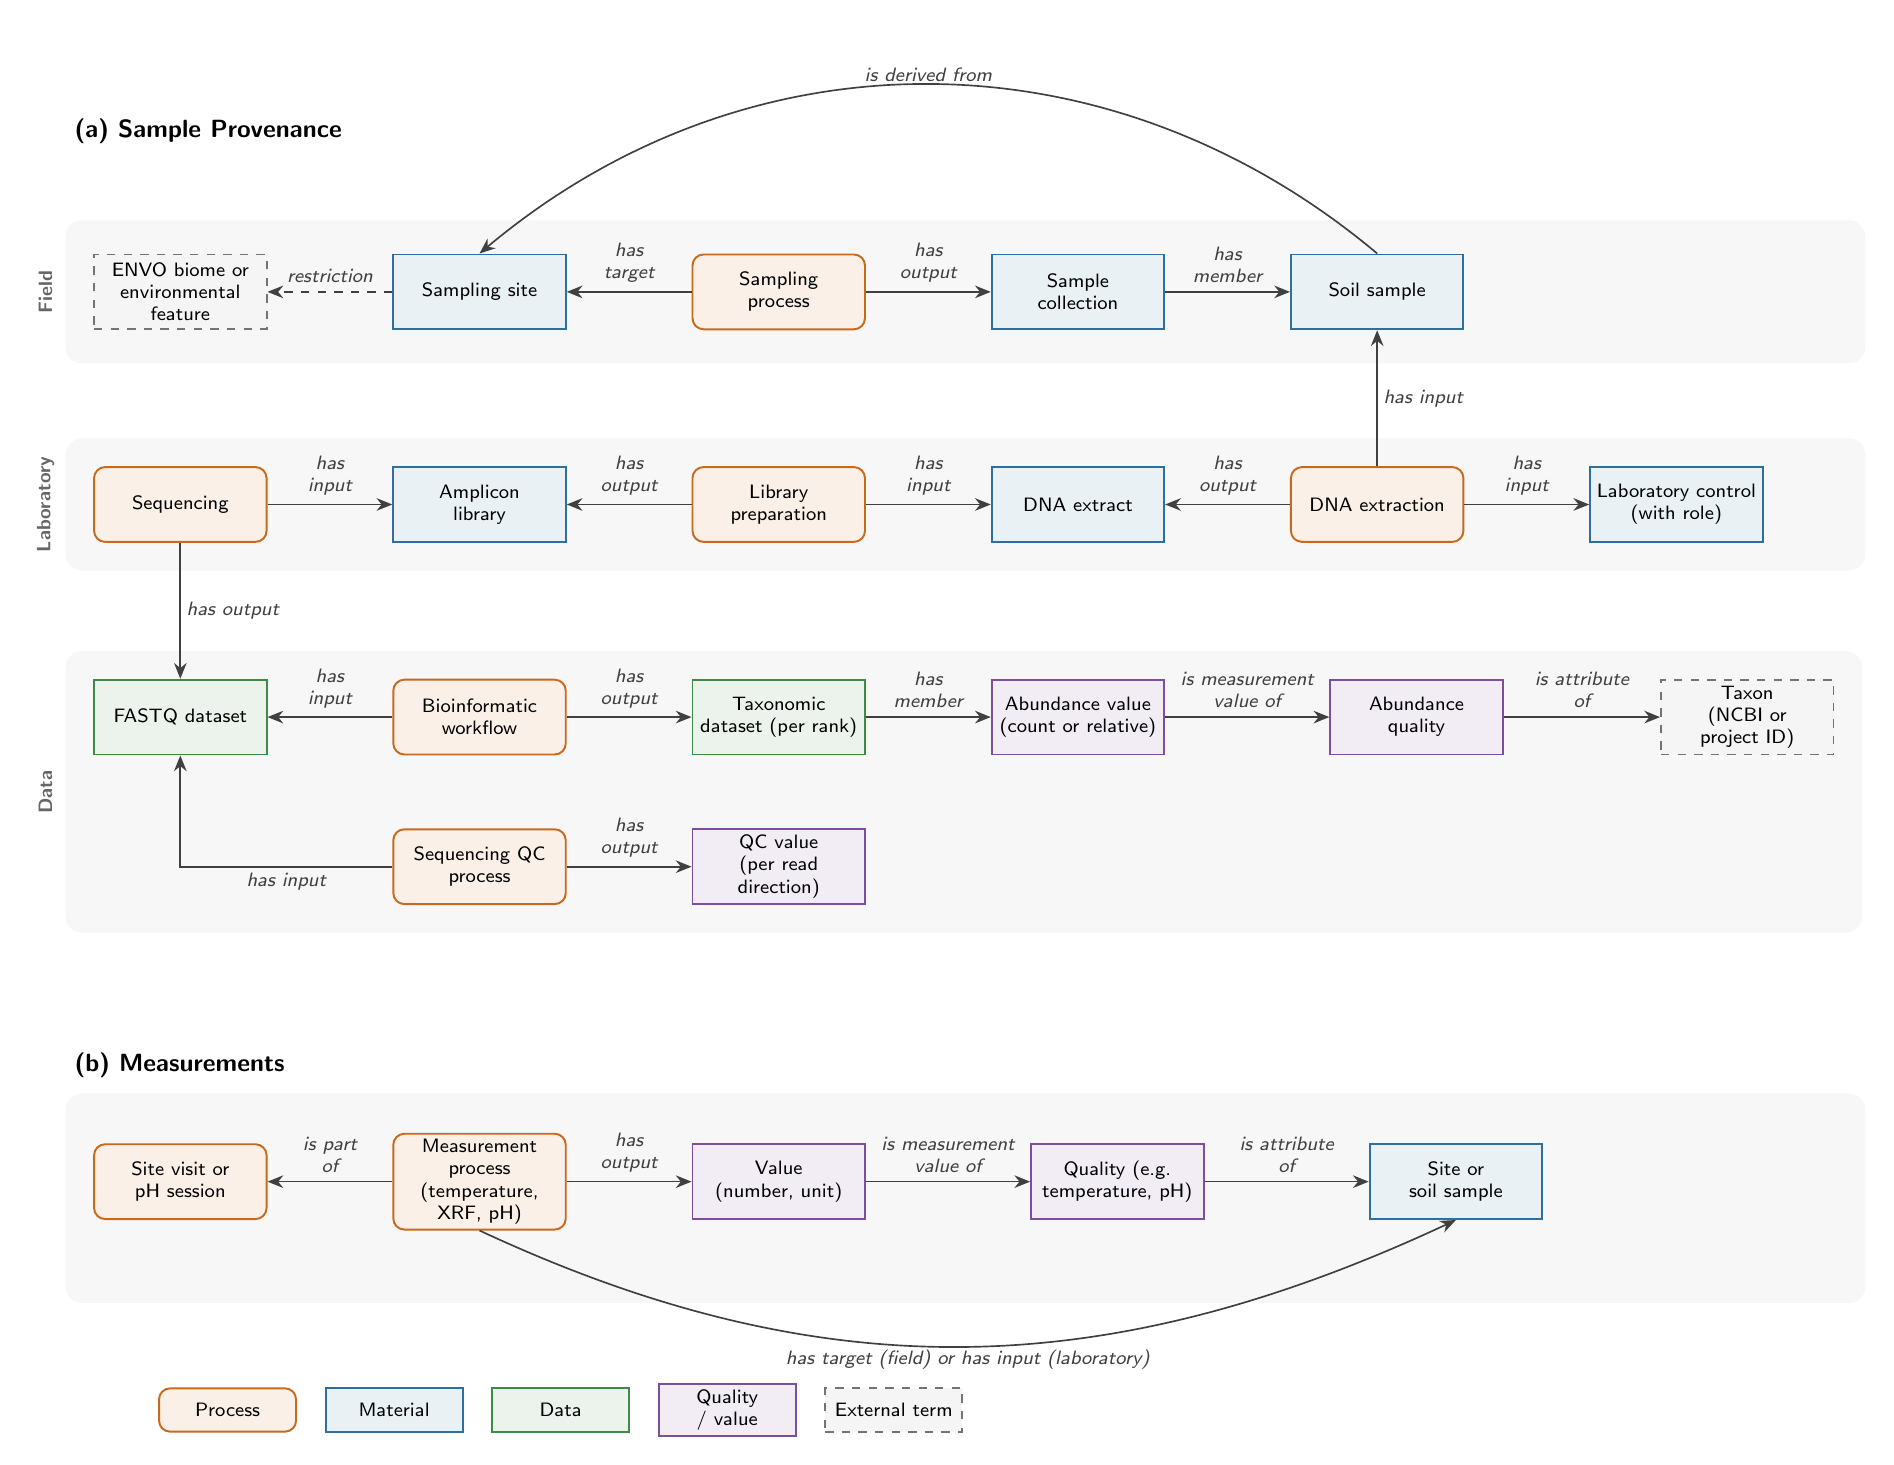
\begin{tikzpicture}[
  font=\sffamily\scriptsize,
  box/.style={draw, line width=0.7pt, text width=2.05cm, align=center,
              minimum height=0.95cm, inner sep=2pt},
  proc/.style={box, draw=kgproc, fill=kgproc!10, rounded corners=4pt},
  mat/.style={box, draw=kgmat, fill=kgmat!10},
  data/.style={box, draw=kgdata, fill=kgdata!10},
  qual/.style={box, draw=kgqual, fill=kgqual!10},
  ext/.style={box, draw=black!55, dashed, fill=black!4},
  rel/.style={-{Stealth[length=2mm,width=1.6mm]}, line width=0.6pt, black!75},
  lbl/.style={font=\sffamily\scriptsize\itshape, inner sep=1pt, text=black!75, align=center},
  lane/.style={fill=black!3, draw=none, rounded corners=6pt},
  lanelab/.style={font=\sffamily\scriptsize\bfseries, rotate=90, text=black!60},
]

% ---------------- Panel (a): sampling-to-data chain ----------------
\def\dx{3.8}
\def\ya{0}
\def\yb{-2.7}
\def\yc{-5.4}

% Field lane (left to right)
\node[ext]  (envo) at (0,\ya)        {ENVO biome or\\environmental feature};
\node[mat]  (site) at (\dx,\ya)      {Sampling site};
\node[proc] (samp) at (2*\dx,\ya)    {Sampling\\process};
\node[mat]  (coll) at (3*\dx,\ya)    {Sample\\collection};
\node[mat]  (smp)  at (4*\dx,\ya)    {Soil sample};

% Laboratory lane (right to left)
\node[mat]  (ctrl) at (5*\dx,\yb)    {Laboratory control\\(with role)};
\node[proc] (ext)  at (4*\dx,\yb)    {DNA extraction};
\node[mat]  (dna)  at (3*\dx,\yb)    {DNA extract};
\node[proc] (lib)  at (2*\dx,\yb)    {Library\\preparation};
\node[mat]  (amp)  at (\dx,\yb)      {Amplicon\\library};
\node[proc] (seq)  at (0,\yb)        {Sequencing};

% Data lane (left to right)
\node[data] (fq)   at (0,\yc)        {FASTQ dataset};
\node[proc] (wf)   at (\dx,\yc)      {Bioinformatic\\workflow};
\node[data] (tds)  at (2*\dx,\yc)    {Taxonomic\\dataset (per rank)};
\node[qual] (aval) at (3*\dx,\yc)    {Abundance value\\(count or relative)};
\node[qual] (aq)   at (4*\dx+0.5,\yc)    {Abundance\\quality};
\node[ext]  (tax)  at (5*\dx+0.9,\yc)    {Taxon\\(NCBI or project ID)};

% QC branch
\node[proc] (qc)   at (\dx,\yc-1.9)  {Sequencing QC\\process};
\node[qual] (qcv)  at (2*\dx,\yc-1.9){QC value\\(per read direction)};

% Lane backgrounds
\begin{scope}[on background layer]
  \coordinate (fr) at ([xshift=2.05cm]5*\dx,\ya);
  \node[lane, fit=(envo)(fr), inner xsep=10pt, inner ysep=12pt] (L1) {};
  \coordinate (lr) at ([xshift=2.05cm]5*\dx,\yb);
  \node[lane, fit=(seq)(ctrl)(lr), inner xsep=10pt, inner ysep=10pt] (L2) {};
  \node[lane, fit=(fq)(tax)(qc)(qcv), inner xsep=10pt, inner ysep=10pt] (L3) {};
\end{scope}
\node[lanelab] at ([xshift=-7pt]L1.west) {Field};
\node[lanelab] at ([xshift=-7pt]L2.west) {Laboratory};
\node[lanelab] at ([xshift=-7pt]L3.west) {Data};

% Field edges
\draw[rel, dashed] (site) -- node[lbl, above=2pt] {restriction} (envo);
\draw[rel] (samp) -- node[lbl, above=2pt] {has\\target} (site);
\draw[rel] (samp) -- node[lbl, above=2pt] {has\\output} (coll);
\draw[rel] (coll) -- node[lbl, above=2pt] {has\\member} (smp);
\draw[rel] (smp.north) to[out=140, in=40]
      node[lbl, pos=0.5, above] {is derived from} (site.north);

% Field-to-lab and lab edges
\draw[rel] (ext) -- node[lbl, right=1pt] {has input} (smp);
\draw[rel] (ext) -- node[lbl, above=2pt] {has\\input} (ctrl);
\draw[rel] (ext) -- node[lbl, above=2pt] {has\\output} (dna);
\draw[rel] (lib) -- node[lbl, above=2pt] {has\\input} (dna);
\draw[rel] (lib) -- node[lbl, above=2pt] {has\\output} (amp);
\draw[rel] (seq) -- node[lbl, above=2pt] {has\\input} (amp);

% Lab-to-data and data edges
\draw[rel] (seq) -- node[lbl, right=1pt] {has output} (fq);
\draw[rel] (wf) -- node[lbl, above=2pt] {has\\input} (fq);
\draw[rel] (wf) -- node[lbl, above=2pt] {has\\output} (tds);
\draw[rel] (tds) -- node[lbl, above=2pt] {has\\member} (aval);
\draw[rel] (aval) -- node[lbl, above=2pt] {is measurement\\value of} (aq);
\draw[rel] (aq) -- node[lbl, above=2pt] {is attribute\\of} (tax);
\draw[rel] (qc) -| node[lbl, pos=0.25, below=1pt] {has input} (fq);
\draw[rel] (qc) -- node[lbl, above=2pt] {has\\output} (qcv);

\node[font=\sffamily\small\bfseries, anchor=south west]
      at ([yshift=24pt]L1.north west) {(a) Sample Provenance};

% ---------------- Panel (b): measurement pattern ----------------
\def\yd{-11.3}
\node[proc] (ctx)  at (0,\yd)        {Site visit or\\pH session};
\node[proc] (mp)   at (\dx,\yd)      {Measurement process\\(temperature,\\XRF, pH)};
\node[qual] (val)  at (2*\dx,\yd)    {Value\\(number, unit)};
\node[qual] (q)    at (3*\dx+0.5,\yd)    {Quality (e.g.\\temperature, pH)};
\node[mat]  (bear) at (4*\dx+1.0,\yd)    {Site or\\soil sample};

\begin{scope}[on background layer]
  \coordinate (br) at ([xshift=2.05cm]5*\dx,\yd);
  \node[lane, fit=(ctx)(br), inner xsep=10pt, inner ysep=24pt,
        yshift=-6pt] (L4) {};
\end{scope}

\draw[rel] (mp) -- node[lbl, above=2pt] {is part\\of} (ctx);
\draw[rel] (mp) -- node[lbl, above=2pt] {has\\output} (val);
\draw[rel] (val) -- node[lbl, above=2pt] {is measurement\\value of} (q);
\draw[rel] (q) -- node[lbl, above=2pt] {is attribute\\of} (bear);
\draw[rel] (mp.south) to[out=-25, in=-155]
      node[lbl, pos=0.5, below, align=center]
      {has target (field) or has input (laboratory)} (bear.south);

\node[font=\sffamily\small\bfseries, anchor=south west]
      at ([yshift=2pt]L4.north west) {(b) Measurements};

% ---------------- Legend ----------------
\def\yl{-14.2}
\node[proc, text width=1.6cm, minimum height=0.55cm] (k1) at (0.6,\yl) {Process};
\node[mat,  text width=1.6cm, minimum height=0.55cm, right=0.35cm of k1] (k2) {Material};
\node[data, text width=1.6cm, minimum height=0.55cm, right=0.35cm of k2] (k3) {Data};
\node[qual, text width=1.6cm, minimum height=0.55cm, right=0.35cm of k3] (k4) {Quality / value};
\node[ext,  text width=1.6cm, minimum height=0.55cm, right=0.35cm of k4] (k5) {External term};
\end{tikzpicture}}
\caption{Main patterns in the knowledge graph. (a)~A sampling process
targets a site and produces a collection of soil samples, each also linked
directly to its site. Laboratory processes are connected through their
inputs and outputs, from DNA extraction to sequencing; laboratory controls
enter at the processing step whose role they test. A bioinformatic
workflow converts each FASTQ dataset into taxonomic datasets at seven
ranks, whose values quantify the abundance of taxa identified by NCBI
Taxonomy or project identifiers. Sites are linked to ENVO classes through
existential restrictions (dashed). (b)~Each measurement process produces a
value that quantifies a quality of a site or soil sample, and is part of
a site visit or pH measurement session. Arrows point from subject to
object of each relation. Protocols linked to each process are omitted for
clarity.}
\label{fig:kg_model}
\end{figure}